\section{Metodolog\'ia}

La metodolog\'ia usar es desarrollo evolutivo, se basa en la idea de desarrollar una implementaci\'on inicial, exponi\'enndola a los comentarios del usuario y refin\'andola a trav\'es de las diferentes versiones hasta que se desarrolle un sistema adecuado. Las actividades deespecificaci\'on, desarrollo y validaci\'n se entrelazan en vez de separarse, con una r\'apida retroalimentaci\'on entre estas.Existen dos tipos de desarrollo evolutivo: desarrolloexploratorio y prototipos desechables, utilizaremos el desarrollo exploratorio,donde el objetivo del proceso es trabajar con el usuario (cliente)para explorar sus requerimientos y entregar un sistema final. El sistema evoluciona agregando nuevos atributos propuestos. Ver \ref{fig:metodologia}.


\begin{figure}
\begin{center}
	\label{metodologia}
	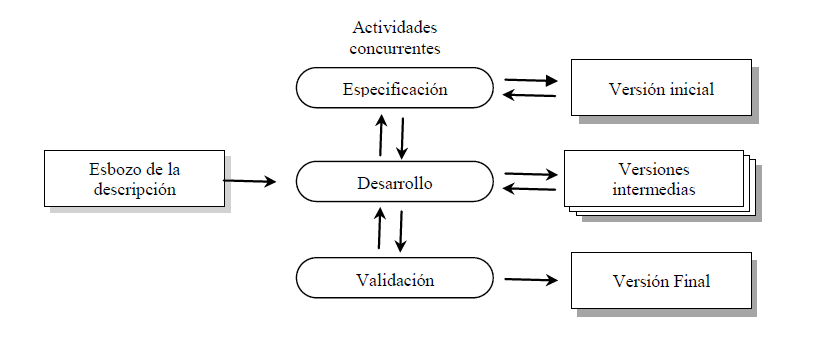
\includegraphics[scale=.6]{images/desarrollo_evolutivo}
	\label{fig:metodologia}
	\caption{Metodolog\'ia}
\end{center}
\end{figure}
